\subsection{Cabling robots}
Cabling robots are systems which use one set of cables to or ensure its proper
positioning in its working area. Cabling robots may have other
adhesion methods technologies in combination with cables.
%São classificados como robôs cabeados quaisquer sistemas robôticos que façam
%uso de um conjunto de cabos e/ou cordas para auxiliar ou mesmo garantir seu
%posicionamento adequado na sua região de trabalho. Sendo assim, robôs cabeados
%podem possuir outros métodos de fixação em conjunto com seu cabeamento.

The cabling system is ideal to applications which robot locomotion is
restricted to a vertical plane and speed velocities are not required. The
cabling system is an weight reduction and manipulator range improvement, or
decrease the adhesion complexity of a climbing robot.
%A idéia do uso de um sistema de cabos surge naturalmente quando o deslocamento
%se mostra majoriamente restrito a um plano vertical e não há exigência de
%grandes velocidades de deslocamento. O sistema é usado como forma de reduzir o
%preso e melhorar o desempenho de um braço mecânico de mesmo alcance, ou
% diminuir a complexidade e a força de aderência necessária para um escalador.

As an example, the \textit{torboMate} is a climber with magnetic
adhesion, can have two or more emitting jets with 4000 bar of supply capacity.
It has 45 kg and reaches 20 m/min speed \citep{torbo}.
%Para exemplificar essa categoria foram selecionados dois robôs. O
%\textit{torboMate} é um escalador que possui adesão magnética que o
%permite caminhar livremente. Pode ter dois ou um
%emissor de jatos com capacidade para abastecimento em até 4000 bar. Possui 45
% kg e atinge uma velocidade de até 20 m/min \citep{torbo}.

\begin{figure}[ht]
	\centering
	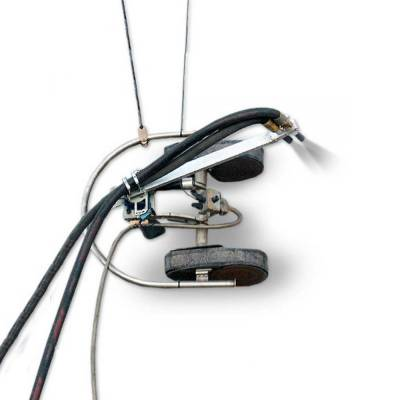
\includegraphics[width=8.4cm]{figs/cables/torbo}
	\caption{TorboMate "Crawler" robot}
	\label{fig:cables:torbo}
\end{figure}

RIWEA is a purely cabling robot, as it has no other type of position
adjustment, for wind power turbines cleaning. It is an open frame concept robot
which uses four ropes to move up and down. It has five main parts automatically
adjust to the blade surface during its move \citep{jeon2012maintenance}.
However, there are chances where RIWEA robot can misjudge contaminated parts of
the blade as cracks. Its greatest strength lies the ability to adapt the
curvature of the blade while maintaining a foothold on it, and it is also less
susceptible to vibration \citep{riwea}.
%RIWEA é um robô puramente cabeado, no sentido em que ele não possui nenhum
%outro tipo de forma de ajuste de posição além do sistema de cabos. É um
%conceito de robô de estrutura aberta que faz uso de quatro cordas para se
%deslocar verticamente \citep{jeon2012maintenance}. Seu maior diferencial reside
%na capacidade de se adaptar a curvatura da pá mantendo sempre um ponto de apoio
%sobre ela, sendo também menos suceptivel a vibrações \citep{riwea}.

\begin{figure}[!h]
	\centering
	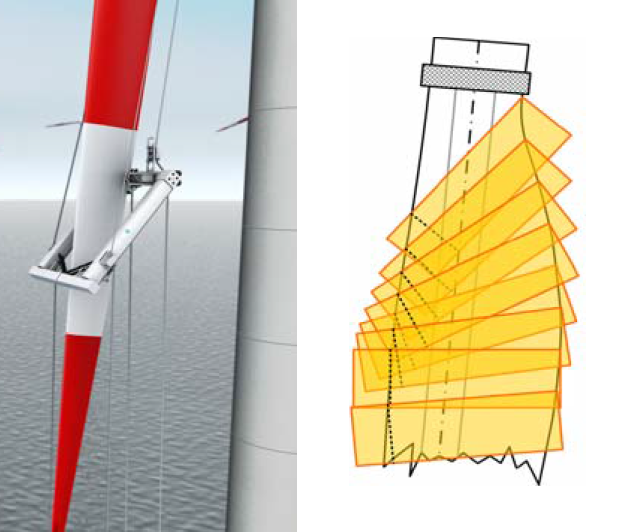
\includegraphics[width=8.4cm]{figs/cables/riwea}
	\caption{RIWEA robot}
	\label{fig:cables:riwea}
\end{figure}

The advantages and disadvantages for cabling robot solutions are:

\textbf{Advantages:}
\begin{itemize}
  \item Load reduction on robot / higher payload capacity.
  \item Robot reach can be extended at low cost.
\end{itemize}

\textbf{Disadvantages:}
\begin{itemize}
  \item Cabling management system complexity.
  \item Need of a superior fixation point for cabling.
\end{itemize}


